%TODO2 To co niżej to nowy rodział (chapter)
%TODO2 Proszę to jeszcze raz wszystko przeczytać !! Bo ja trochę poprzestawiałem....
\chapter{Implementacja i ewaluacja systemu sprzętowo-programowego}
\label{cha:implementacja_systemu}

Na rysunku \ref{fig:system} przedstawiono ogólny schemat zaimplementowanego systemu. 
Na~niebiesko zaznaczone zostały wykorzystywane urządzania, na~żółto oznaczono moduły zaimplementowane w~części rekonfigurowalnej, natomiast na~zielono zaznaczono system procesorowy. 
Sygnał wizyjny z~kamery trafia do~części reprogramowalnej i~jest następnie przetwarzany przez poszczególne moduły. 
Po~wyborze znacznika informacja o~jego pozycji i~uchybie regulacji trafia do~procesora. 
System procesorowy wysyła komendy sterujące do~kontrolera drona. 
Zadaniem układu regulacji jest przesunięcie drona nad~lądowisko, umożliwiając wykonanie lądowania.
W~dalszej części rozdziału omówiono poszczególne komponenty systemu. 

\begin{figure}[h]
	\centering
	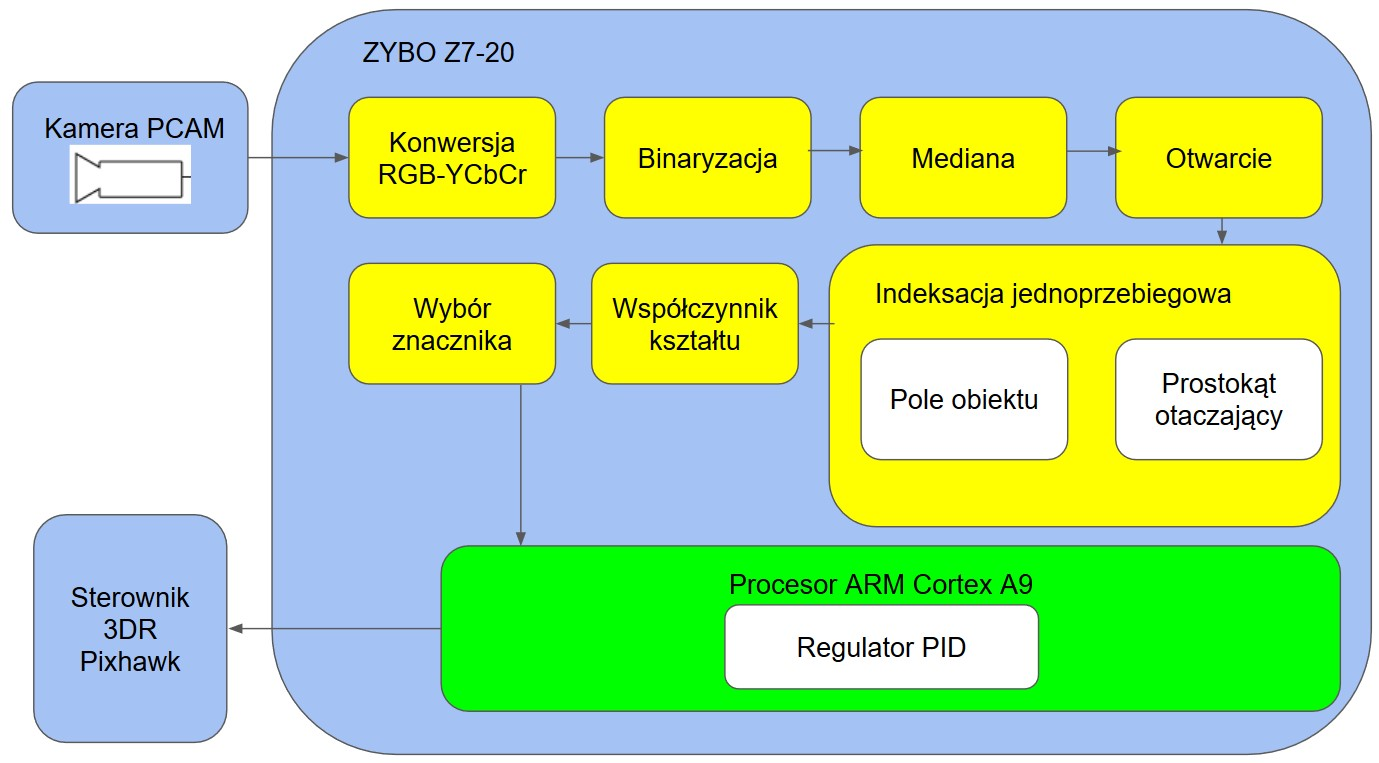
\includegraphics[width=\textwidth]{system.jpg}
	\caption{Schemat przedstawiający zaimplementowany system.}
	\label{fig:system}
\end{figure} 

\section{Akwizycja obrazu}
\label{sec:akwizycja}
Firma Digilent, na swojej stronie internetowej, zapewnia projekt demonstracyjny połączenia kamery i~płytki~\cite{projektPCAM}. 
Pozwala on pobrać obraz z~kamery oraz wyświetlić go na monitorze.
Ponadto, przez port szeregowy możliwa jest zmiana rozdzielczości, szybkości akwizycji ramek, współczynnika korekcji gamma oraz ustawień balansu bieli. 
Możliwe są~następujące opcje dotyczące dwóch pierwszych parametrów:
\begin{itemize}
	\item 1280 x 720, 60 fps,
	\item 1920 x 1080, 15 fps,
	\item 1920 x 1080, 30 fps.
\end{itemize}

Przeprowadzone eksperymenty pokazały, że przy rozdzielczości 1280 x 720 kąt widzenia kamery jest większy. 
Ze tego względu zdecydowano się użyć tej rozdzielczości w~docelowym systemie.
Przeprowadzanie syntezy i~implementacji projektu możliwe było przy użyciu darmowego oprogramowania Vivado oraz SDK w~wersji WebPack (w wersji~2018.2). 
Opisany projekt stanowił bazę do dalszych prac.

\subsection{Zapis ramek na kartę SD}
\label{sec:image_sd}
%TODO2 Do tego ma się znaleźć link w tej części o modelu !!!(wykonane)
Aby możliwe było użycie ramek z kamery w~modelu programowym, należało zaimplementować akwizycję obrazów na~kartę~SD. 
W~użytym projekcie bazowym zastosowano połączenie toru wizyjnego AXI z~zewnętrzną pamięcią RAM dostępną na karcie Zybo poprzez moduł \textit{AXI Video Direct Memory Access}. 
%Informacja o~adresie pamięci, gdzie zapisywane są~ramki, podawana jest przy inicjalizacji połączenia na~terminal. 
%TODO2 to jest niejasne.(poprawione poniżej)
Szesnastkowy adres miejsca w~pamięci, gdzie znajduje się wartość składowej R pierwszego piksela ramki, przesyłany jest do~użytkownika przy inicjalizacji połaczenia. Możliwe jest jego odczytanie i~dotarcie do~zawartości pamięci przy wykorzystaniu wskaźnika w~języku~C++.

W~celu umożliwienia komunikacji z~kartą SD uaktywniono interfejs procesora SD0. 
Następnie do~projektu w~SDK dodano bibliotekę ,,xilffs'' i~korzystając z~funkcji systemu plików opisanych w~\cite{xilffs}, zaimplementowano zapis ramek obrazu do~pliku. 
Ze~względu na~prostotę pliku zdecydowano~się na~format ppm. 
W~formacie tym nie występuje kompresja i~przez to jest on~nieefektywny pod~względem zapotrzebowania na pamięć.
Niemniej jednak, dysponując odpowiednio dużą ilością miejsca na~karcie i~chcąc w~łatwy sposób zapisać dane, warto zastosować właśnie ten format. 
Zapis danych w~formacie ppm jest prosty, gdyż plik składa się jedynie z~nagłówka (typ pliku, rozmiary obrazka, maksymalna wartość składowych) oraz kolejnych wartości w~formie pojedynczych bajtów (jeśli maksymalna wartość jest mniejsza niż 256).  



\section{Podłączenie laserowego czujnika wysokości}
\label{subsec:podlaczenie_lasera}

Czujnik wysokości podłączono z~zastosowaniem wyjścia PWM (ang. \textit{Pulse-Width Modulation}). %TODO2 a) rozwinąć skrót, b) w opisie sprzętu zaznaczyć, że są dwie możliwości (wykonane)
W~tym trybie czujnik ustawia stan wysoki na~wyjściu przez czas proporcjonalny do~zmierzonej odległości. 
Stan wysoki trwa 10~\si{\micro\second} na~każdy zmierzony centymetr. 
Pin wyzwalania zwarto na~stałe do~masy, powodując ciągłe wykonywanie pomiaru. 
Wyjście PWM podłączono do~trzeciego pinu portu Pmod~JB układu ZYBO. %TODO2 skoro tak, to znowu w opisie sprzętu trzeba zaznaczyć, co to jest PMod (wykonane)
Okazało się, że~możliwe jest działanie modułu przy zasilaniu bezpośrednio z~płytki z napięciem 3,3~V.

Moduł odczytujący wysokość zaimplementowany został jako maszyna stanów. 
Stan pierwszy to~oczekiwanie na~pojawienie się stanu wysokiego. 
Po~wykryciu zbocza narastającego następuje zerowanie rejestrów oraz przejście do~stanu drugiego. 
W~tym stanie liczony jest czas trwania stanu wysokiego. 
Wywoływanie procesu z~częstotliwością 1~MHz, czyli co~1~\si{\micro\second} pozwala na~łatwą konwersję zmierzonego czasu na~odległość. 
Odczytana wysokość jest następnie przesyłana do~procesora z~użyciem rejestrów~AXI.


\section{Konwersja z przestrzeni barw RGB do YCbCr}
\label{subsec:konwersja}
Konwersję z przestrzeni barw RGB do YCbCr wykonano zgodnie ze wzorem \ref{eq:ycbcr}. 
Przy implementacji wykorzystano sprzętowe mnożarki oraz sumatory. 
Na~rysunku \ref{fig:drzewo_ycbcr} przedstawiono schemat operacji arytmetycznych dla jednej ze~składowych. 
Aby możliwe było prowadzenie obliczeń, wszystkie stałe należało przedstawić w~postaci liczb stałoprzecinkowych. 
Do~reprezentacji stałoprzecinkowej użyto rejestrów o~szerokości 18~bitów.
\begin{equation}
\label{eq:ycbcr}
\begin{bmatrix} Y \\ 
Cb\\
Cr
\end{bmatrix}=
\begin{bmatrix} 0,299 & 0,587 & 0,114\\ 
-0,168736 & -0,331264 & 0,5\\
0,5 & -0,418688 & 0,081312
\end{bmatrix}
\begin{bmatrix} R\\
G\\
B
\end{bmatrix}+
\begin{bmatrix} 0\\
128\\
128
\end{bmatrix}
\end{equation}


\begin{figure}[h]
	\centering
	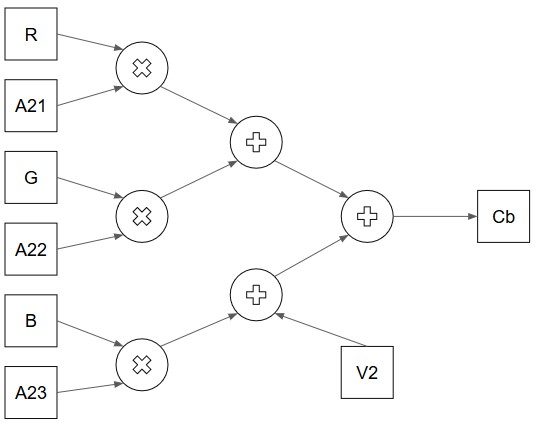
\includegraphics[width=0.7\textwidth]{drzewo_ycbcr.jpg}
	\caption{Schemat wyznaczania składowej Cb. $A21=-0,168736, A22=-0,331264, A23=0,5, V2=128$.}
	\label{fig:drzewo_ycbcr}
\end{figure} 

\section{Binaryzacja}
\label{subsec:Binaryzacja}
% dobieranie progu: 2 multiplekser sterowany buttonem?
Piksel wyjściowy otrzymywał wartość maksymalną (kolor biały), jeśli wartości Cb i~Cr mieściły się pomiędzy wyznaczonymi eksperymentalnie progami.  
W~innym przypadku pikselowi przypisywana była wartość 0 (kolor czarny). 
Do~szybkiej zmiany progów wykorzystano komunikację PS-PL z~użyciem rejestrów AXI -- progi mogły być zmieniane z~poziomu terminala i~testy nie wymagały ponownych implementacji projektu.  


\section{Mediana}
\label{subsec:Mediana}
% obrazek wyznaczania kontekstu
% obrazek drzewa sumacyjnego

W~przypadku działania na~obrazie binarnym operacja mediany może być przeprowadzona przez obliczenie sumy wartości pikseli wewnątrz kontekstu, a~następnie porównanie jej z~połową maksymalnej wartości tej sumy. 
Ze względu na łatwość implementacji oraz zadowalające wyniki filtracji, zdecydowano się na~rozpatrywanie kontekstu w~kształcie kwadratu o~boku 5~pikseli. 
Spowodowało to~konieczność zapamiętywania kontekstu piksela w~25 rejestrach oraz 4~linii obrazu w~długich liniach opóźniających zbudowanych w~oparciu o~pamięć BRAM.
Schemat wyznaczania kontekstu przedstawiono na rysunku \ref{fig:kontekst}. 
Sygnały synchronizacji zostały doklejone do wartości piksela i~w~przedstawionej strukturze przesuwają się razem z~nim. 
Sumę wyliczano w~2~etapach, dodając najpierw elementy w~wierszach, potem sumując wyniki (Rys. \ref{fig:drzewo_sumacyjne}).

\begin{figure}[h]
	\centering
	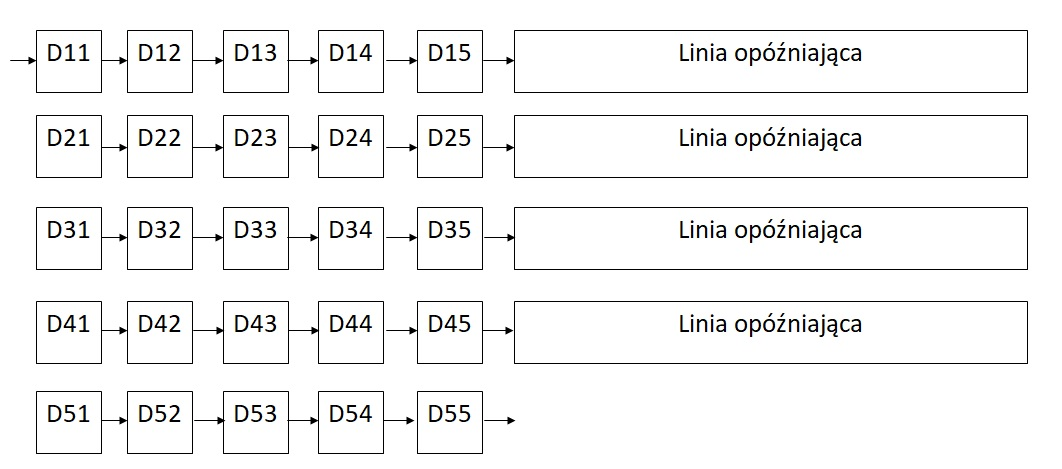
\includegraphics[width=0.8\textwidth]{kontekst.jpg}
	\caption{Schemat wyznaczania kontekstu dla mediany, erozji i dylatacji.}
	\label{fig:kontekst}
	%TODO2 nieco mniejszy ten rysunek (wykonane)
\end{figure}  

\begin{figure}[h]
	\centering
	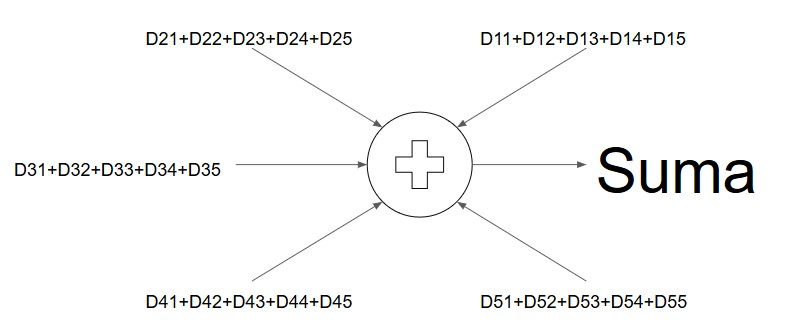
\includegraphics[width=\textwidth]{drzewo_sumacyjne.jpg}
	\caption{Schemat wyznaczania sumy otoczenia piksela.}
	\label{fig:drzewo_sumacyjne}
\end{figure}  

\section{Otwarcie}
\label{subsec:erozja}

Moduł erozji ustawia wartość piksela wyjściowego na~maksymalną wartość, gdy~w~sąsiedztwie znajdują się same białe piksele. 
W~module dylatacji zwracana jest wartość maksymalna, gdy~przynajmniej jeden piksel w~sąsiedztwie ma~wartość maksymalną.
Podobnie jak w~przypadku mediany, jako element strukturalny zdecydowano się na~kwadrat o~boku 5~pikseli i~zastosowano rozwiązanie podobne jak przy medianie (Rys. \ref{fig:kontekst}).
%TODO2 Tu jakieś zdanie, że zostaosowano podobne rozwiązanie jak przy medianie (wykonane)

%TODO2 Teraz patrząc na schemat to indeksacja.
\section{Indeksacja}
\label{subsec:indeksacja}

Zazwyczaj na wejście modułu indeksacji podawany jest obraz zbinaryzowany, natomiast na~wyjściu pojawia się obraz, na którym  wartość  pikseli odpowiada przypisanej do~danego obiektu etykiecie. 
Rozważane jest otoczenie każdego piksela, składające się z trzech pikseli nad nim oraz jednego po~lewej stronie, tak jak zostało to przedstawione na rysunku \ref{fig:ind_sasiedztwo}. 
Indeksacji dokonuje się bezpośrednio na~obrazie wejściowym. 
Podczas iteracji po wszystkich pikselach, w~przypadku znalezienia piksela należącego do któregoś z~obiektów, może zajść jeden z~trzech przypadków:
\begin{enumerate}[label=(\alph*)]
	\item w~otoczeniu piksela znajdują się tylko piksele należące do tła,
	\item otoczenie zawiera jeden lub więcej pikseli, którym została wcześniej przypisana taka sama etykieta~$L$,
	\item w~otoczeniu znajdują się piksele posiadające różne etykiety (np. $L1$ i $L2$).
\end{enumerate} 
\begin{figure}[h]
	\centering
	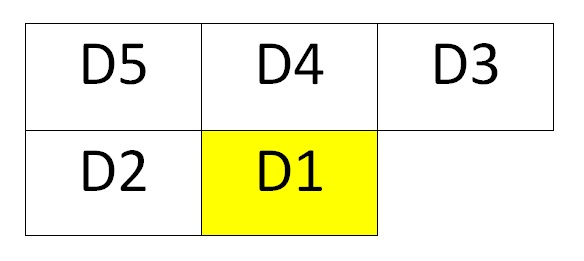
\includegraphics[width=0.5\textwidth]{ind_sasiedztwo.jpg}
	\caption{Sąsiedztwo piksela brane pod uwagę przy indeksacji}
	\label{fig:ind_sasiedztwo}
\end{figure}

W~pierwszym przypadku pikselowi zostaje przypisana nowa etykieta. 
Gdy spełniony jest warunek $b$, punkt otrzymuje etykietę $L$, natomiast jeśli zachodzi przypadek $c$, przypisywana jest mniejsza z~etykiet. 
W~ten sposób otrzymuje się obraz wstępnie poetykietowany. 
Najczęściej posiada on więcej przypisanych etykiet, niż obiektów. 
Dlatego istnieje konieczność złączenia ze~sobą pewnych etykiet przy użyciu tablicy sklejeń. 
Tablica ta zawiera informację, które etykiety powinny zostać złączone. 
W~przypadku~$a$ do tablicy sklejeń na~pozycji odpowiadającej etykiecie zapisywana jest etykieta, natomiast gdy zachodzi opcja~$c$ etykietę mniejszą zapisuje się pod indeksem większej. 
Należy zaznaczyć, że opisana wersja obsługi sklejeń działa poprawnie tylko w~przypadku braku tzw. ,,łańcuchów sklejeń'' tj. dla uproszczonych kształtów. %TODO2 Proszę mieć tego świadomość !
Do sklejenia etykiet potrzebna jest druga iteracja, tym razem po~obrazie wstępnie poetykietowanym.

Powyższy fakt jest główną przeszkodą w~łatwym wykonaniu takiego algorytmu w~systemie potokowym. 
Bez~zapamiętywania całej ramki, w~przypadku sklejania etykiet, niemożliwy jest powrót do~wcześniej przetwarzanych pikseli. 
Pomimo tego, możliwe jest obliczenie pewnych cech obiektów, takich jak: pole, współrzędne środka ciężkości, prostokąt otaczający. 
W~pracy \cite{COG} podano sposób, w~jaki można tego dokonać. 
Opiera się on~na~scaleniu nie samych wartości pikseli, ale~obliczanych na~bieżąco parametrów obiektu.
Implementacja indeksacji w~języku Verilog rodzi trudności związane z~określeniem przypadku istnienia tej~samej lub~różnych etykiet w~otoczeniu piksela. 

O~ile~wykrycie przypadku $a$ jest łatwe, to~przypadki $b$~i~$c$ wymagały rozważenia kilku możliwości. 
Zdecydowano się na~wykrywanie ich za~pomocą flag bitowych. 
Na~ich podstawie wnioskowano o~zachodzącym aktualnie przypadku oraz wskazywano, od~którego piksela z~otoczenia powinna zostać przepisana etykieta. 
Zgodnie z~opisanymi wcześniej zasadami uzupełniano również tablicę sklejeń.
Oprócz tego, na bieżąco obliczano prostokąt otaczający oraz liczbę pikseli należących do~każdego ze~znalezionych obiektów. 


Po poetykietowaniu całej ramki obrazu wykorzystano tablicę sklejeń do~złączenia obliczanych na~bieżąco cech. 
Ten~etap algorytmu zaimplementowano jako maszynę stanów:
\begin{itemize}
	\item Stan 0 -- Oczekiwanie na sygnał końca ramki wyznaczany na podstawie synchronizacji pionowej. W~momencie wykrycia sygnału następuje rejestrowanie tablicy sklejeń i~obliczonych parametrów (w~następnym takcie zostaną one zresetowane), zerowanie tablic wypełnianych w~kolejnym etapie oraz przejście do~stanu~1. 
	\item Stan 1 -- Iteracja po tablicy sklejeń i~uzupełnianie rzeczywistych wartości cech obiektów.
	\item Stan 2 -- Uporządkowanie tablic z~wyznaczonymi parametrami.
	\item Stan 3 -- Obliczenie pola prostokąta otaczającego dla każdego znalezionego obiektu. Wykorzystywana jest mnożarka o~latencji 3.
	\item Stan 4 -- Szukanie obiektu spełniającego warunki minimalnej wielkości pola powierzchni oraz stosunku pola prostokąta otaczającego do pola obiektu.
\end{itemize}
Schemat przetwarzania danych po~każdej ramce pokazano na rysunku \ref{fig:ind_schemat}.
\begin{figure}[h]
	\centering
	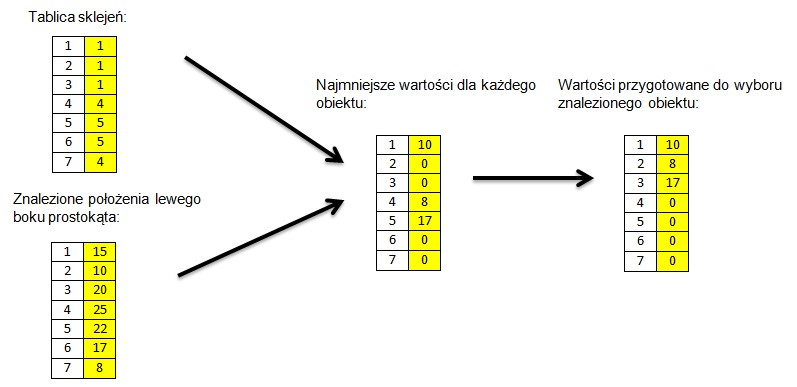
\includegraphics[width=\textwidth]{ind_schemat.jpg}
	\caption{Schemat procesu przetwarzania informacji po~każdej ramce obrazu przy zastosowaniu indeksacji z~przykładowymi danymi. Tablica sklejeń daje informację o~konieczności sklejenia etykiet 1, 2, 3. Ponieważ przykład dotyczy lewego boku prostokąta, spośród liczb 15, 10, 20 (odpowiadającym etykietom 1, 2, 3) wybierana jest najmniejsza. Ostatni krok przetwarzania to~usunięcie środkowych zer z~wektora.}
	\label{fig:ind_schemat}
\end{figure}


Główną trudnością w~implementacji opisanego algorytmu w~układzie FPGA jest stosunkowo duże zapotrzebowanie na~zasoby sprzętowe. 
Należy zarezerwować miejsce na~cechy każdego potencjalnego obiektu. 
Ogranicza to~liczbę możliwych etykiet. 
Zasoby części rekonfigurowalnej układu dostępnego na karcie ZYBO~Z7-20 pozwoliły na~zarezerwowanie miejsca dla~30~etykiet. 
Przy pewnej określonej orientacji znacznika nie jest to~niestety wystarczająca liczba etykiet (Rys. \ref{fig:rezultaty_ind}). %TODO2 może przykład (zdjęcie) i komentarz 
\begin{figure}
	\centering
	\begin{subfigure}{0.45\textwidth}
		\centering
		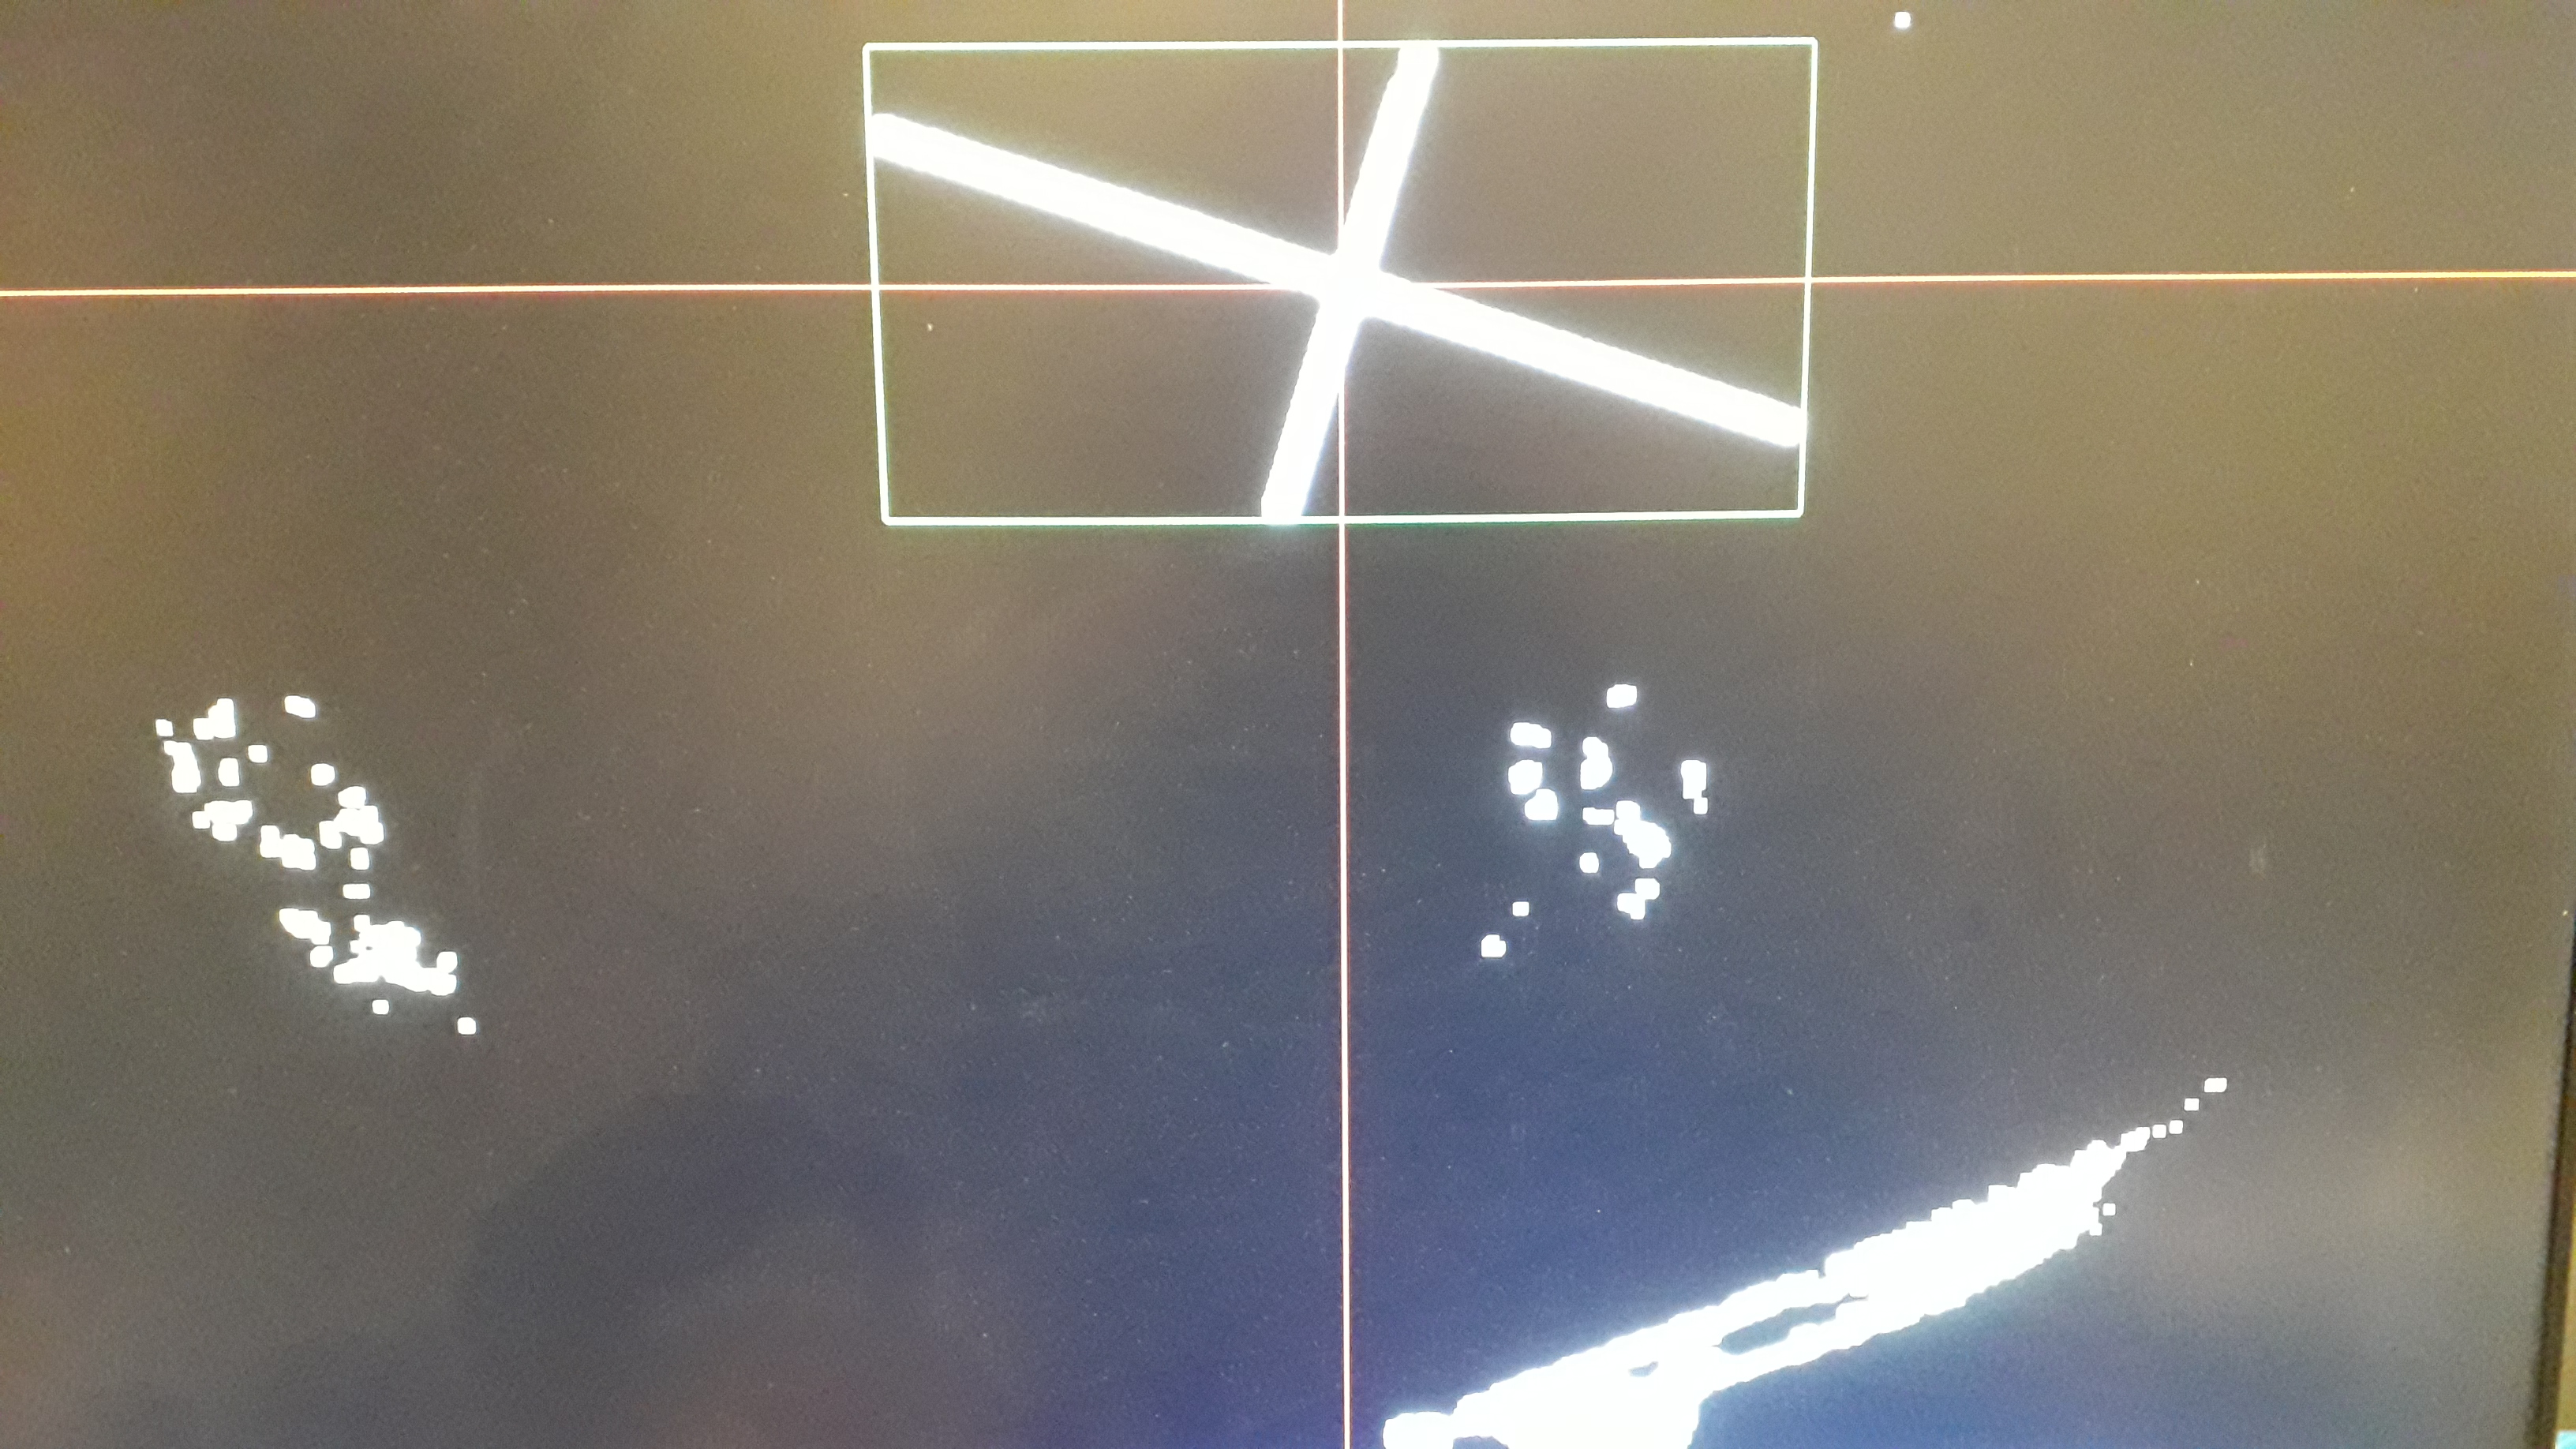
\includegraphics[width=\textwidth]{ind_poprawna.jpg}
		\caption{Poprawne wykrycie znacznika}
		\label{fig:ind_poprawna}
	\end{subfigure}
	\begin{subfigure}{0.45\textwidth}
		\centering
		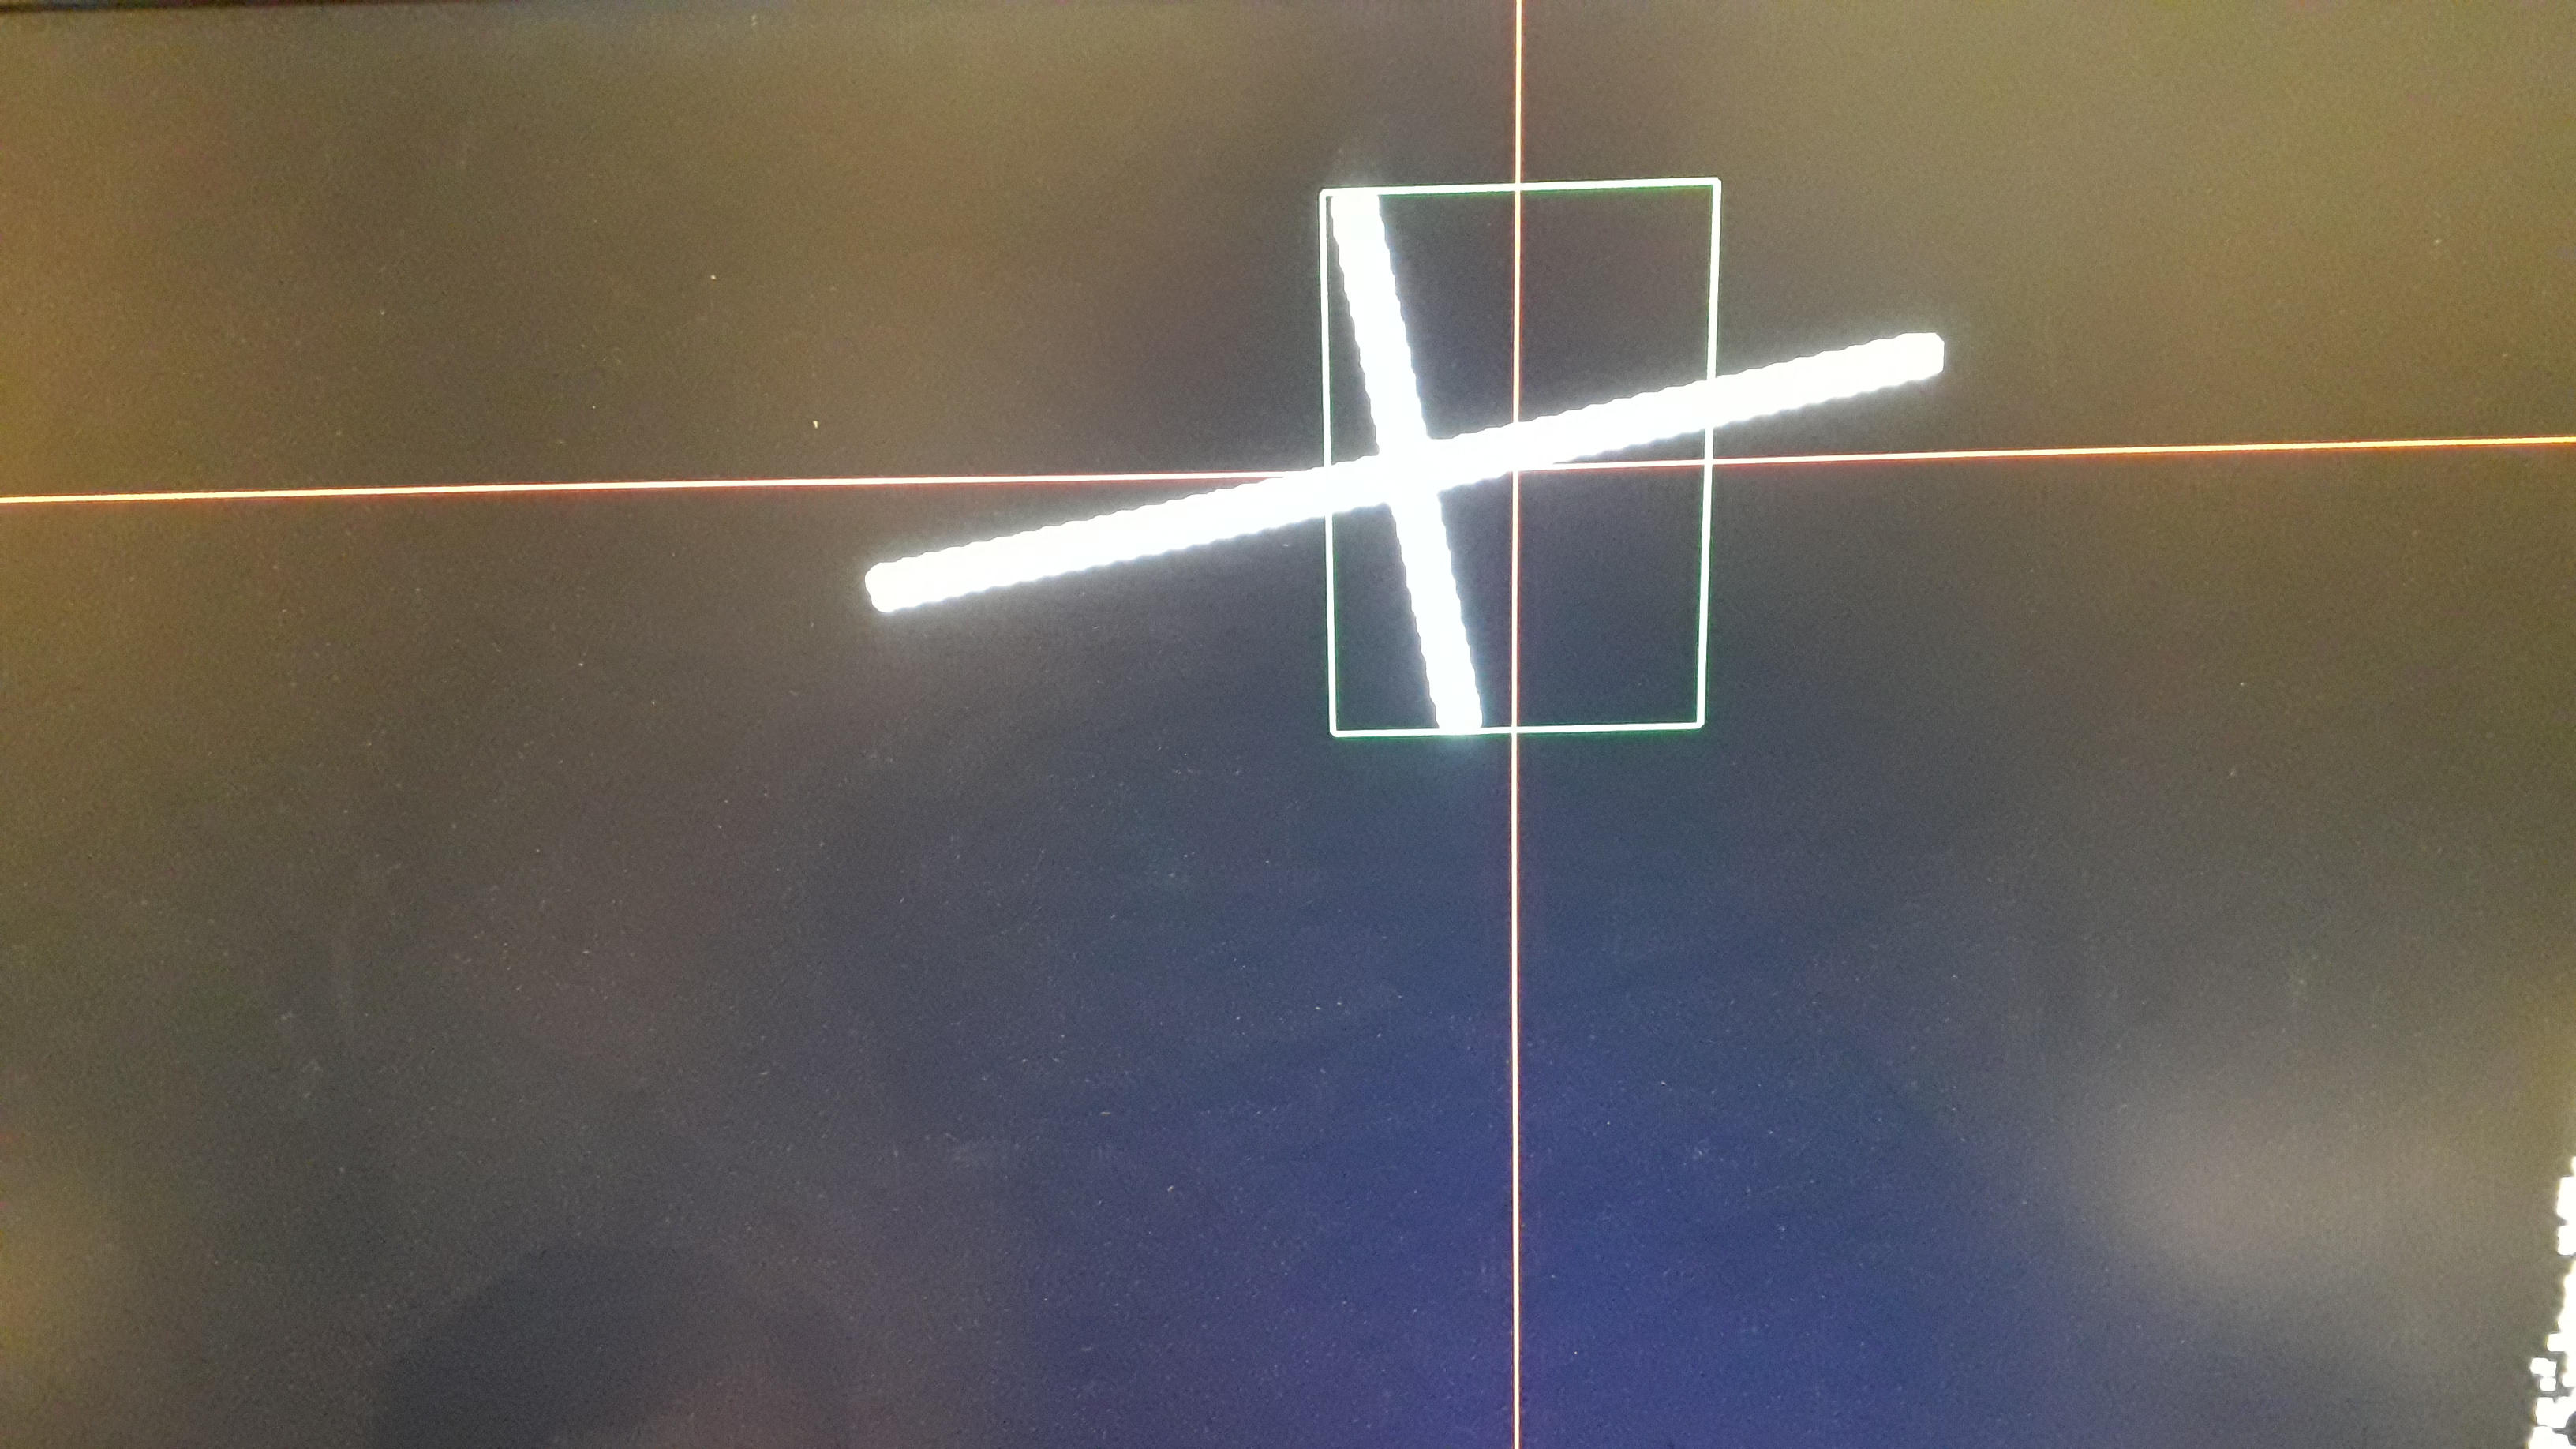
\includegraphics[width=\textwidth]{ind_niepoprawna.jpg}
		\caption{Obcięcie części znacznika ze~względu na brak etykiet}
		\label{fig:ind_niepoprawna}
	\end{subfigure}\\
	\caption{Rezultaty indeksacji w~zależności od~orientacji znacznika}
	\label{fig:rezultaty_ind}
\end{figure}
Aby możliwa była sprawna detekcja miejsca lądowania niezależnie od~orientacji markera, należało zmienić nieco koncepcję systemu. 
Innym podejściem było obliczanie środka ciężkości wszystkich białych pikseli. 
Eliminuje to~możliwość klasyfikacji obiektów ze~względu na~kształt (pozostaje klasyfikacja po~kolorze) i~tym samym czyni system podatnym na~zakłócenia. 
Pojawienie się w~kadrze innych grup pikseli o~tym samym kolorze spowoduje przesunięcie środka ciężkości.
Jednak w~warunkach testowych możliwe jest wypełnienie powierzchni kolorem silnie kontrastującym z~barwą znacznika. 
Z~tego powodu moduł wyznaczający środek ciężkości (podrozdział \ref{subsec:srodek_ciezosci}) był wykorzystywany podczas testowania rozwiązania.
Wyznaczanie pola figury i~prostokąta otaczającego (podrozdział \ref{subsec:prostokat_otaczajacy}) umożliwiało odrzucanie pewnych detekcji i~wysyłanie sygnału o~braku znalezienia znacznika. 
%TODO2 do tego akapitu powyżej proszę dopisać zdanie polu i prostokącie otaczającym oraz odwołać się do tych podrozdziałów poniżej. (wykonane)

\section{Wyznaczanie środka ciężkości}
\label{subsec:srodek_ciezosci}

Do wyznaczania środka ciężkości pikseli należących do~obiektu wykorzystano wzory \eqref{eq:m00}, \eqref{eq:m10} i~\eqref{eq:m01}.

\begin{equation}
\label{eq:m00}
m_{00}=\sum_{i=0}^{N-1}\sum_{j=0}^{M-1} x_{ij}
\end{equation}
\begin{equation}
\label{eq:m10}
m_{10}=\sum_{i=0}^{N-1}\sum_{j=0}^{M-1} i*x_{ij}
\end{equation}
\begin{equation}
\label{eq:m01}
m_{01}=\sum_{i=0}^{N-1}\sum_{j=0}^{M-1} j*x_{ij}
\end{equation}
gdzie:
\begin{eqwhere}[2cm]
	\item[$N$] szerokość obrazu w pikselach,
	\item[$M$] wysokość obrazu w pikselach,
	\item[$x_{ij}$] wartość piksela o~współrzędnych $i$, $j$ obrazu zbinaryzowanego.
\end{eqwhere}
Na ich podstawie obliczono środek ciężkości przy zastosowaniu wzorów \eqref{eq:xsc} i~\eqref{eq:ysc}.
\begin{equation}
\label{eq:xsc}
X_{sc}=\frac{m_{10}}{m_{00}}
\end{equation}
\begin{equation}
\label{eq:ysc}
Y_{sc}=\frac{m_{01}}{m_{00}}
\end{equation}
gdzie:
\begin{eqwhere}[2cm]
	\item[$X_{sc}$] współrzędna pozioma środka ciężkości,
	\item[$Y_{sc}$] współrzędna pionowa środka ciężkości.
\end{eqwhere}

W~module na podstawie sygnałów synchronizacji oraz wymiarów obrazka wyznaczono współrzędne aktualnie przetwarzanego piksela. 
Jeśli jest to piksel należący do obiektu, następuje zwiększenie wartości odpowiednich rejestrów zgodnie ze wzorami
\ref{eq:m00}, \ref{eq:m10} i~\ref{eq:m01}. 
Po przejściu przez całą ramkę obrazu wykonywane jest dzielenie na podstawie wzorów \ref{eq:xsc} i~\ref{eq:ysc}.

\subsection{Wyznaczanie prostokąta otaczającego i~pola powierzchni}
\label{subsec:prostokat_otaczajacy}

Znalezienie prostokąta otaczającego sprowadza się do wyznaczenia skrajnych jego punktów na górze, dole, po lewej oraz prawej stronie. 
Na podstawie sygnałów synchronizacji oraz wymiarów obrazka wyznaczano współrzędne aktualnie przetwarzanego piksela. 
Jeśli jest to piksel należący do obiektu, następuje inkrementacja jego pola powierzchni. 
Do~odpowiednich rejestrów trafiają wówczas również wartości współrzędnych piksela, jeśli wykraczają poza aktualną zawartość rejestrów:
\begin{itemize}
	\item do~rejestru zawierającego górny bok prostokąta trafi współrzędna wierszowa, jeśli będzie ona mniejsza od aktualnej,
	\item do~rejestru zawierającego dolny bok prostokąta trafi współrzędna wierszowa, jeśli będzie ona większa od aktualnej,
	\item do~rejestru zawierającego lewy bok prostokąta trafi współrzędna kolumnowa, jeśli będzie ona mniejsza od aktualnej,
	\item do~rejestru zawierającego prawy bok prostokąta trafi współrzędna kolumnowa, jeśli będzie ona większa od aktualnej,
\end{itemize}  
%Obliczeń pola powierzchni i~współrzędnych prostokąta otaczającego nie~wykonywano w~oddzielnym module, lecz stanowiły one część modułu indeksacji.
%TODO 2 indekacji czy tej analizy bez indekacji... bo teraz jest zamieszanie. 


\section{Algorytm sterowania}
\label{sec:algorytm_sterowania}

Informacjami o~detekcji lądowiska, koniecznymi do~realizacji algorytmu sterowania, są:
\begin{itemize}
	\item uchyb regulacji w~obu osiach, rozumiany jako odległość środka obrazu od~środka wykrytego lądowiska (centrum prostokąta otaczającego lub środka ciężkości),
	\item wiadomość o~znalezieniu znacznika. %TODO2 niestosowanie indeksacji nie wyklucza analizy kształtu (za małe pole, czy proporporcjie i może tego sygnału nie być)
\end{itemize}
%TODO2 tu jakaś informacja o tym, jak ta informacja jest przesyłana z PL do PS(wykonane)
Informacje te przesyłano z~części rekonfigurowalnej do~systemu procesorowego przy wykorzystaniu rejestrów AXI.

Dodatkowo, w~celu analiza działania systemu, istnieje możliwość podglądu przetworzonego obrazu na~monitorze, podłączonym poprzez port HDMI. 
Możliwy jest podgląd kolejnych etapów przetwarzania -- wybór etapu następuje przez zmianę ustawień przełączników na~płytce.

Algorytm sterowania bazuje na~dyskretnym regulatorze PID, zrealizowanym w~systemie procesorowym układu.
Regulacji podlegają składowe $x$ i~$y$ wektora położenia drona względem znacznika określającego lądowisko. 
Jeśli znacznik zostanie utracony z~pola widzenia kamery na~czas 1~sekundy, dron przechodzi w~tryb unoszenia się nad ziemią.

\section{Integracja płytki z autopilotem}
\label{sec:integracja_plytka_autopilot}

W~układzie Zynq z~karty ZYBO~Z7-20 wykorzystano interfejs UART0. 
Wyprowadzono piny TX i~RX z~systemu procesorowego i~podłączono je do~portu Pmod~JB. 
Po~stronie sterownika Pixhawk użyto portu TELEM~2. 
Szybkość transmisji to~115200~bodów.

Wysyłanie komend opiera się na~wykorzystaniu gotowych funkcji dostępnych w~sieci \cite{github_mavlink}.
Przygotowują one daną wiadomość zgodnie z~wymaganiami protokołu MAVLink. 
Następnie wywoływane są funkcje wysyłające przygotowaną tablicę bajtów przez odpowiedni UART. 
W~projekcie wykorzystano stworzone przy wykonywaniu pracy \cite{mgr} funkcje opakowujące kolejne etapy przetwarzania komend.
\section{Ewaluacja}
\label{sec:ewaluacja_sprzetu}
%TODO 2 Wtępniak
Zaimplementowane rozwiązania należało przetestować. Eksperymentem pozwalającym sprawdzić działanie laserowego czujnika odległości, przetwarzania wizyjnego i~algorytmu sterującego był test opisany w~podrozdziale \ref{sec:test_sterowania}. Test ten wymagał również integracji urządzeń na~platformie. Podrozdział \ref{sec:test_autopilota} opisuje natomiast test komunikacji karty i~sterownika drona. 
\subsection{Test sterowania}
\label{sec:test_sterowania}

Test ten polegał na ,,ręcznym'' wykonywaniu komend pochodzących z systemu procesorowego -- dron był trzymany w~ręce. 
Zaplanowano 3 fazy lotu: wznoszenie na określoną wysokość, kierowanie drona w~stronę znacznika oraz lądowanie.
Przy takim rozwiązaniu niemożliwe było zadawanie prędkości wynikającej z~regulacji PID. 
Ograniczono się do wysyłania komend: ,,w górę'', ,,w lewo'', ,,do przodu'' itp. 
Postarano się, aby podłoże miało kolor niebieski, kontrastujący z~czerwoną barwą znacznika. 
Zdjęcie z~eksperymentu przedstawiono na~Rys. \ref{fig:eksperyment}.\\
Test wykazał prawidłowe działanie laserowego czujnika odległości. 
Poprawnie podawane były również komendy dotyczące zmiany pozycji drona. 
\begin{figure}[h]
	\centering
	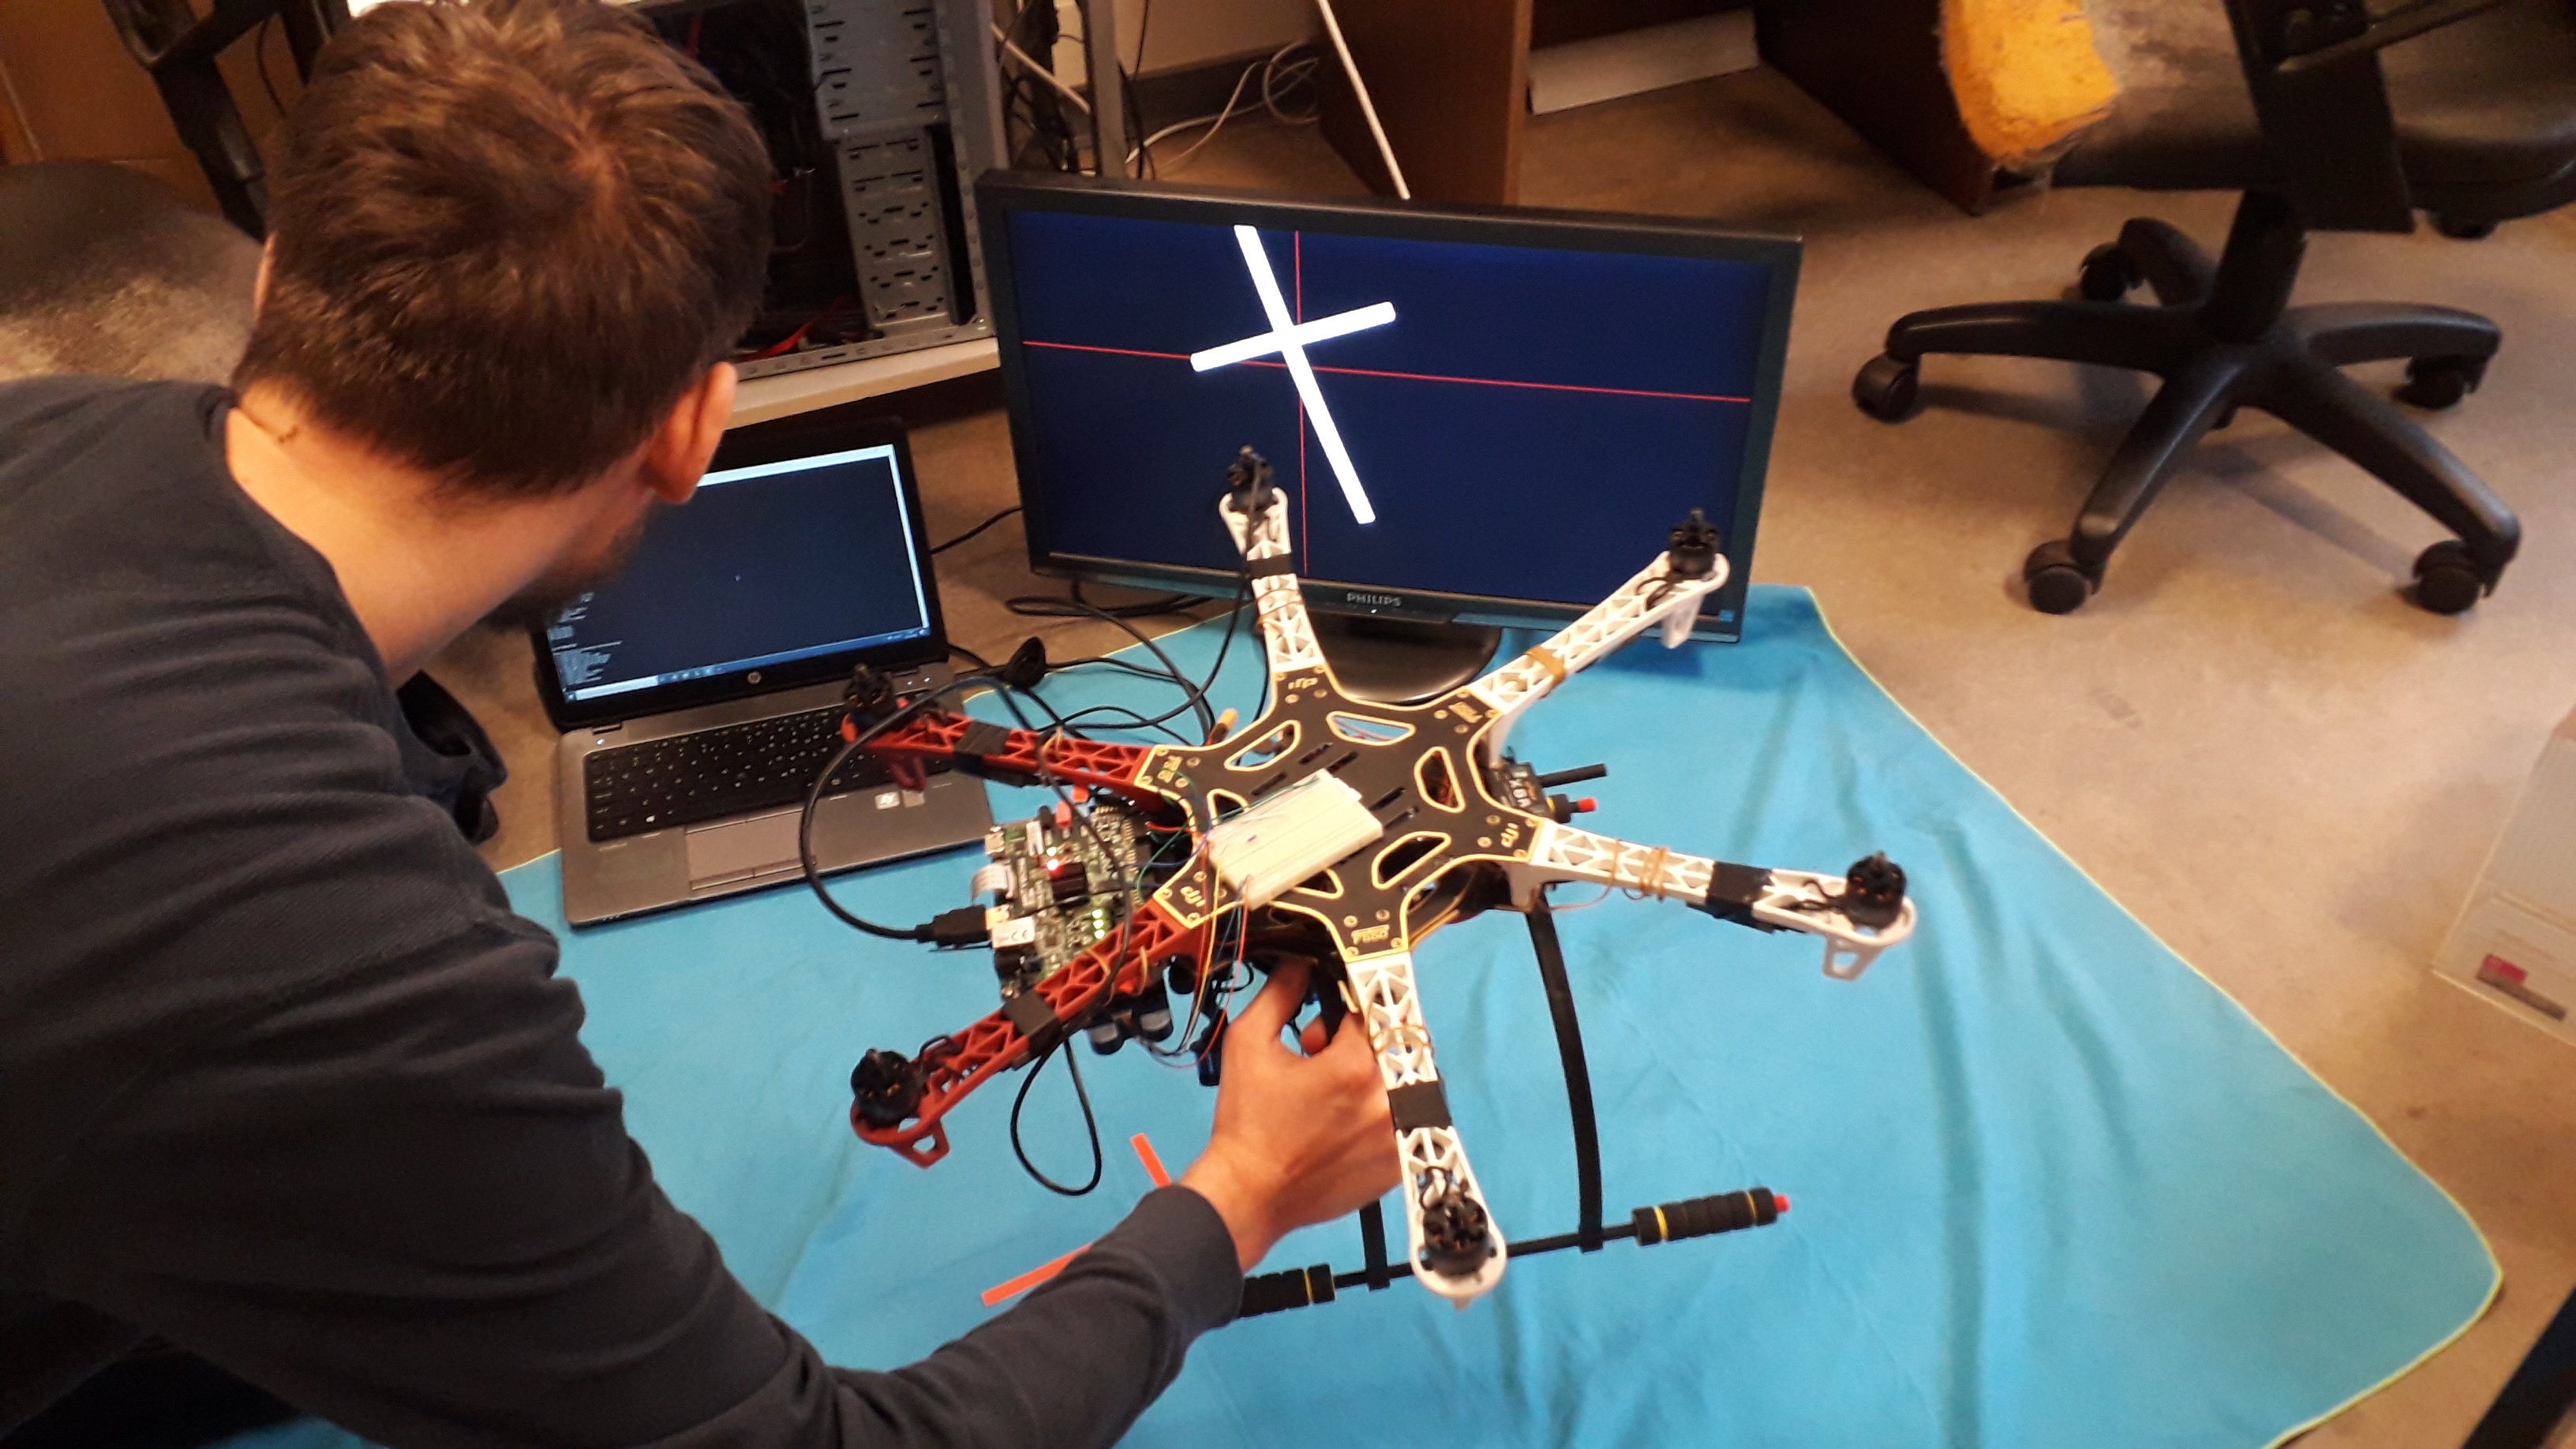
\includegraphics[width=\textwidth]{eksperyment.jpg}
	\caption{Zdjęcie z~eksperymentu. Kartę ZYBO~Z7-20 zamontowano z~przodu platformy. Poniżej umieszczono kamerę i~Lidar. Na~górze znajduje się płytka prototypowa do~łatwego łączenia komponentów.}
	\label{fig:eksperyment}
\end{figure}
\subsection{Test reakcji autopilota na zadawane komendy}
\label{sec:test_autopilota}
Test polegał na~wysyłaniu do~autopilota komend z~karty ZYBO~Z7-20. %TODO2 ZYBO to karta, układ to Zynq - proszę na to zwrócić uwagę.(wykonane)
Podczas eksperymentu śmigła drona były zdjęte. 
Wewnątrz budynku, możliwe było wysłanie komendy uzbrojenia silników w~trybie \textit{Stabilize}. 
Jak opisano w~rozdziale \ref{sec:autopilot}, nie jest to jednak tryb pozwalający na~wysyłanie komend ruchu.
Aby możliwe było kierowanie dronem, należało przeprowadzić eksperyment na~zewnątrz, w~celu utrzymania dostatecznie silnego sygnału GPS. 
Po~uaktywnieniu trybu \textit{Guided} wysłano kolejno komendy uzbrojenia silników, startu i~lotu z~określoną prędkością. 
Silniki reagowały na~wysyłane rozkazy.

Po~eksperymencie można było wysnuć wniosek o~poprawnej konfiguracji komunikacji pomiędzy kartą ZYBO, a~sterownikiem Pixhawk.

\section{Podsumowanie}
%TODO2 kilka słów o testach + jeszcze o komunikacji RF - nawet jak nie zadziałała
Test sterowania pokazał możliwość wykrycia lądowiska i~obliczania takiego sterowania dronem, aby lądowanie odbyło się w~wyznaczonym miejscu. Test komunikacji ze~sterownikiem pozwolił natomiast potwierdzić, że poprawnie utworzone zostało połączenie między platformą obliczeniową, a~autopilotem. 
